\section{Theorie}
\label{sec:Theorie}

\subsection{Quantenzahlen in Atomen}
\noindent Die Elektronenkonfigurationen in den Atomhüllen werden über die Quantenzahlen
$n$, $l$, $m$ beschrieben,
wobei $n$ die Anregungszustände der Elektronen beschreibt.
Die Quantenzahl $l$ beschreibt den Bahndrehimpuls der Elektronen 
und liegt zwischen $0$ und $n-1$. 
Die magnetische Quantenzahl $m$ liegt im Intervall $\left[-l,l \right]$.
Der Spin $S$ ist für Elektronen $1 / 2$ oder $- 1 / 2$.
Der Atomkern besitzt ebenfalls einen Kernspin $I$.
Für \ce{^{85}Rb} ist $I_{\ce{^{85}Rb}}=5 / 2$
und für \ce{^{87}Rb} ist  $I_{\ce{^{87}Rb}}=3 / 2$.
\newline \newline
\noindent Mit diesen Quantenzahlen lässt sich die Aufspaltung der Energieniveaus,
die durch verschiedene Effekte entsteht, beschreiben.
Die schematische Darstellung ist in Abbildung \ref{fig:Energieniveaus} zusehen.

\begin{figure}
    \centering
    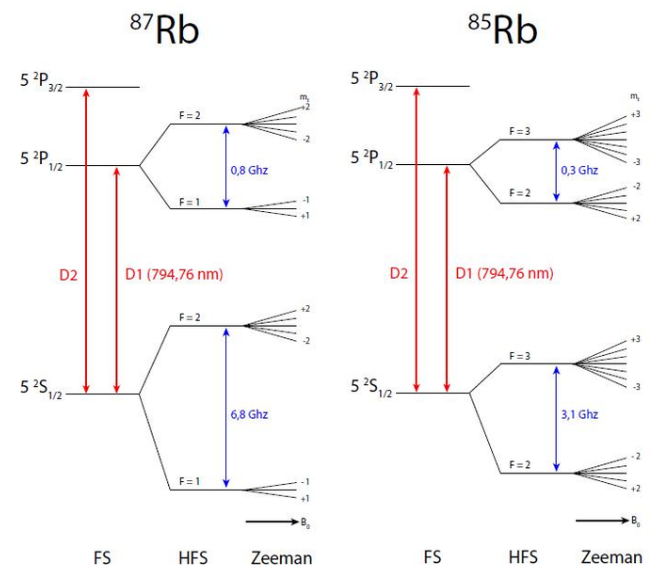
\includegraphics[width=\textwidth]{Fotos/energieniveaus.png}
    \caption{Eine schematische Darstellung der Auspaltung von den Energieniveaus für 
    \ce{^{85}Rb} und für \ce{^{87}Rb} \cite{energieniveaus}.}
    \label{fig:Energieniveaus}
\end{figure}

\subsection{Die Feinstrucktur}
\noindent Die Feinstrucktur (FS) entsteht durch die Kopplung des Bahndrehimpuls $L$ 
und dem Spin $S$. 
Diese koppeln, da 
-aus dem Ruhesystem des Elektrons gesehen-
sich das Elektron in einem Magnetfeld, 
das durch den umkreisenden Atomkern entsteht, befindet
und dieses Magnetfeld mt dem magnetischen Moment des Spins interagiert.
Die Kopplung lässt sich mit dem Gesammtdrehimpuls $J$ beschreiben:
$J= | L + S |$ 
oder 
$J= | L - S |$.

\subsection{Die Hyperfeinstrucktur}
\noindent Da der Atomkern einen Kernspin $I$ besitzt und somit ein magnetisches Moment,
werden -ähnlich wie bei der Spin-Bahn-Kopplung-
das Kernspin $I$ und der Gesammtdrehimpuls $J$ gekoppelt.
Dadurch entsteht die Hyperfeinstrucktur und weitere Aufspaltung der Energieniveaus.
Für diese gilt $F= | I + J |$ oder $F= | I - J|$.

\subsection{Der (quadratische) Zeemann-Effekt}
\noindent Wenn ein äußeres Magnetfeld angelegt wird, 
spalten sich die Energieniveaus weiter auf.
Dieser Prozess wird Zeemann-Effekt genannt.
Durch ihre Kreisbahn besitzen die Elektronen ein magnetisches Moment:
\begin{equation}
    \mu_b = \frac{e \hbar}{2 m_e},
\end{equation}
\noindent wobei $e$ die Elementarladung,
$\hbar$ das Planksche Wirkungsquantum und
$m_e$ die Elektronmasse ist.
Die Aufspaltung entsteht, 
weil ich das magnetische Moment im B-Feld neu ausrichtet:
\begin{equation}
   \Delta E_Z = g_F \mu_b B.
\end{equation}

\noindent Der Landé’schen G-Faktor $g_F$ ist abhängig 
von $S$,$L$ und $I$:
\begin{equation}
    g_F= g_J \frac{F \left( F + 1 \right) + J \left( J + 1 \right) 
    - I \left( I + 1 \right)}
    {2 F \left( F + 1 \right)}  \quad \text{mit}
\end{equation}
\begin{equation}
    g_J = 1 + \frac{J \left( J + 1 \right) + S \left( S + 1 \right) 
    - L \left( L + 1 \right)}
    {2 J \left( J + 1 \right)}.
\end{equation}

\noindent Bei hohen Magnetfeldstärken gilt der quadratische Zeemann-Effekt:
\begin{equation}
    \Delta E_Z = g_F \mu_b B +  
    \left(g_F \mu_b B \right)^2 \frac{1 -2 M_F}{\Delta E_\text{Hyp}}.
\end{equation}
\noindent $\Delta E_\text{Hyp}$ ist die Energiedifferenz,
die durch die Hyperfeinstrucktur entsteht.

\subsection{Optisches Pumpen}
\begin{figure}[h!]
    \centering
    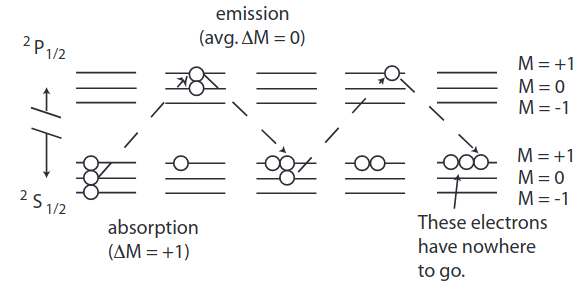
\includegraphics[width=0.85\textwidth]{Fotos/pumpen.png}
    \caption{Eine schematische Darstellung 
    des optischen Pumpens bei Wasserstoff \cite{pumpen_caltech}.}
    \label{fig:pumpen}
\end{figure}

Unter optischem Pumpen wird verstanden,
wenn mithilfe von Licht eine Besetzungsinversion erzeugt wird.
Damit ist gemeint, 
dass mehr Elektronen sich in höheren Energiezuständen befinden 
als im thermichen Gleichgewicht.
Bei der Anregung der Elektronen 
durch polarisiertes Licht werden Übergangsregens beachtet:
Bei Anregung mit rechts-zirkulär polarisiertem Licht gilt $\Delta m = +1$,
mit links-zirkulär polarisiertem $\Delta m = -1$
und mit linear polarisiertem $\Delta m = 0$.
Wird ein das Atom, 
das durch den Zeemann-Effekt in den Energieniveaus gespalten ist,
lange genug mit zirkulär polarisiertem Licht angeregt,
sammeln sich die Elektronen auf der untersten Schale mit höhsten $m$-Wert,
weil sie dort nicht mehr angeregt werden können. 
Es werden keine weiteren Photonen absorbiert 
und der Stoff wird transparent.
In Abbildung \ref{fig:pumpen} ist der Vorgang des Pumpens dargestellt.
\newline \newline

\noindent Durch das Anlegen eines RF-Feldes lässt das Absorptionsverhalten des Stoffes ändern.
Wird das Magnetfeld zum Erzeugen des Zeemann-Effektes ausgeschalltet oder das den
Elektronen mit dem RF-Feld die Energiedifferenz zwischen den Zuständen hingefügt,
können diese wieder in die niedrigeren Zustände übergehen.
Somit können Photonen erneut absorbiert werden (siehe Abbildung \ref{fig:trans}).

\begin{figure}
    \centering
    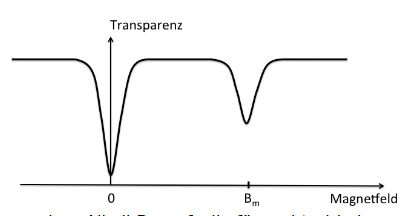
\includegraphics[width=0.80\textwidth]{Fotos/trans.png}
    \caption{Die Tranparenz des Stoffes in Abhängigkeit des angelegten B-Feldes 
    mit $B_m = \frac{\hbar \omega_\text{RF}}{g_F \mu_b }$ \cite{V21}.}
    \label{fig:trans}
\end{figure}

\subsection{Transiente Effekte}
\noindent Ist die RF-Frequenz auf die Resonanz eingestellt 
und wird schnell aus und abgeschaltet,
ist eine Schwingung in der Transparenz zu sehen. 
Über die Periodendauer $T=\frac{1}{\gamma B_\text{RF}}$ 
(mit $\gamma = g_F \frac{\mu_b}{h}$) lässt sich das Verhältnis
\begin{equation}
    \frac{T_85}{T_87} = \frac{\gamma_85}{\gamma_87}
\end{equation}
\noindent herleiten.



